\documentclass{standalone}
\usepackage{tikz}

\begin{document}

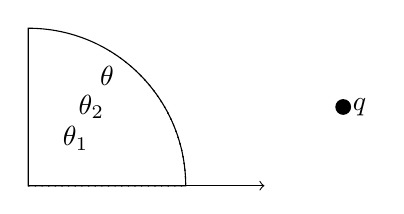
\begin{tikzpicture}[scale=2]
    % Draw the outer arc
    \draw (0,0) -- (1,0) arc (0:90:1) -- cycle;
    
    % Draw the inner arcs
    \draw[dotted] (0,0) -- (1,0) arc (0:45:1);
    \draw[dotted] (0,0) -- (1,0) arc (0:60:1);
    
    % Label the angles
    \node at (0.5,0.7) {$\theta$};
    \node at (0.3,0.3) {$\theta_1$};
    \node at (0.4,0.5) {$\theta_2$};
    
    % Draw the arrow
    \draw[->] (1,0) -- (1.5,0);
    
    % Draw the point q
    \fill (2,0.5) circle (0.05) node[right] {$q$};
\end{tikzpicture}

\end{document}